\section{Exercise 02}
\subsection{}

\begin{frame}
\frametitleTC{Problem}
\framesubtitleTC{This one we solve together}
\myPause
 Take the same system as in exercise 01, i.e.,
 \begin{displaymath}
  A = \begin{bmatrix} 0.4 & 0.4 \\ 0.05 & 0.3 \end{bmatrix}, \quad
  b = \begin{bmatrix} 1 \\ 0.5 \end{bmatrix}, \quad
  c = \begin{bmatrix} 2 & -1 \end{bmatrix}, \quad
  d = 0,
 \end{displaymath}
 and turn it into a block diagram.\\ \myPause
 \vspace{5mm}Important hint: since $z$ is the one-step advance operator, $z^{-1}$ is the one-step\\
 \emph{delay} operator, i.e., 
 \begin{displaymath}
  z^{-1} v(k) = v(k-1).
 \end{displaymath}
\end{frame}

\begin{frame}
\frametitleTC{Solution}
\framesubtitleTC{}
\myPause
 \only<2 >{One delay element per state variable:\\
           \begin{center}
            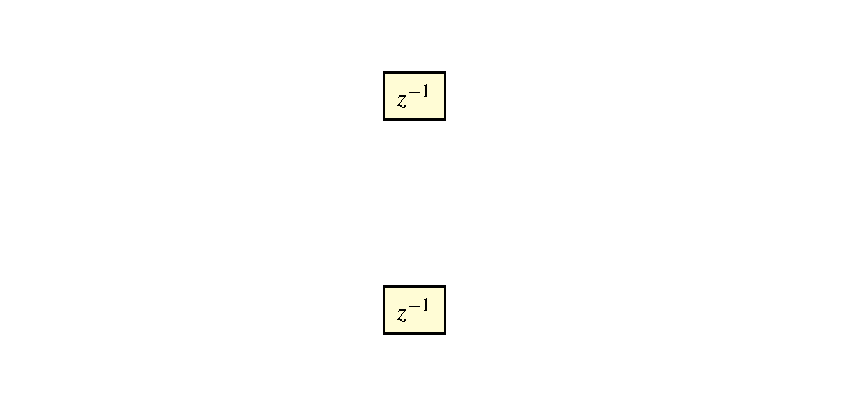
\includegraphics[width=0.85\columnwidth]{./Unit-03/img/PS01-ex02-fig01.pdf}
           \end{center}}
 \only<3 >{If the inputs are the $x_i(k+1)$, then the outputs are the $x_i(k)$:\\
           \begin{center}
            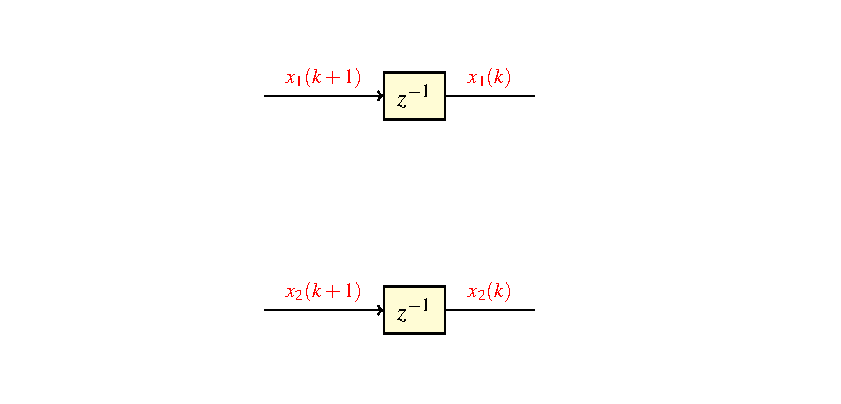
\includegraphics[width=0.85\columnwidth]{./Unit-03/img/PS01-ex02-fig02.pdf}
           \end{center}}
 \only<4 >{Now place the elements of \textcolor{magenta}{$A$} and \textcolor{blue}{$b$}:\\
           \begin{center}
            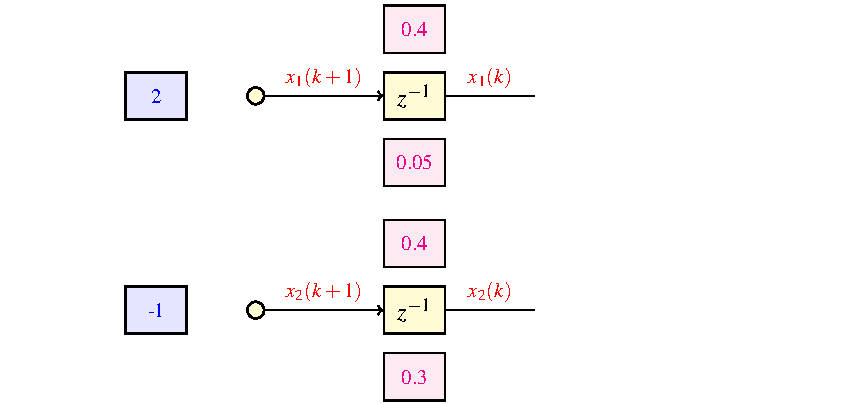
\includegraphics[width=0.85\columnwidth]{./Unit-03/img/PS01-ex02-fig03.pdf}
           \end{center}}
 \only<5 >{Read the state equation and wire how $x(k+1)$ depends on $x(k)$:\\
           \begin{center}
            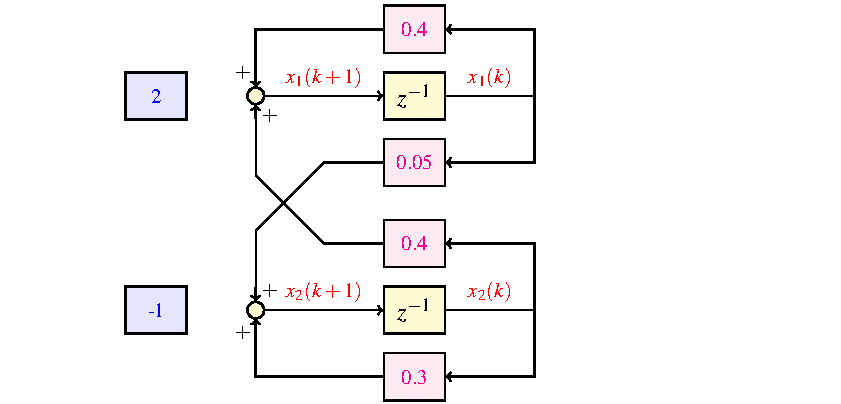
\includegraphics[width=0.85\columnwidth]{./Unit-03/img/PS01-ex02-fig04.pdf}
           \end{center}}
 \only<6 >{Continue reading and wire how $x(k+1)$ depends on $u(k)$:\\
           \begin{center}
            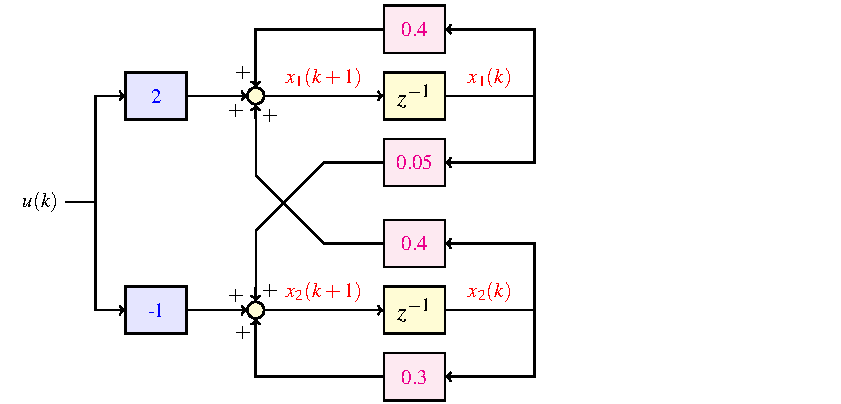
\includegraphics[width=0.85\columnwidth]{./Unit-03/img/PS01-ex02-fig05.pdf}
           \end{center}}
 \only<7 >{Now place the elements of \textcolor{green!80!black}{$c$}:\\
           \begin{center}
            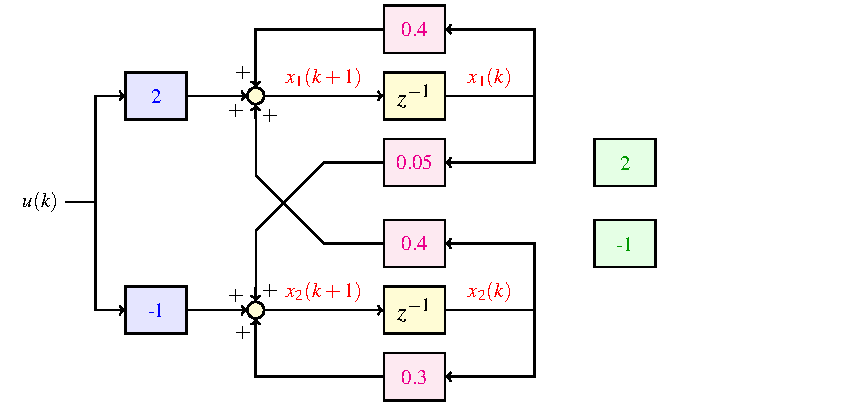
\includegraphics[width=0.85\columnwidth]{./Unit-03/img/PS01-ex02-fig06.pdf}
           \end{center}}
 \only<8->{Read the output equation and complete the block diagram:\\
           \begin{center}
            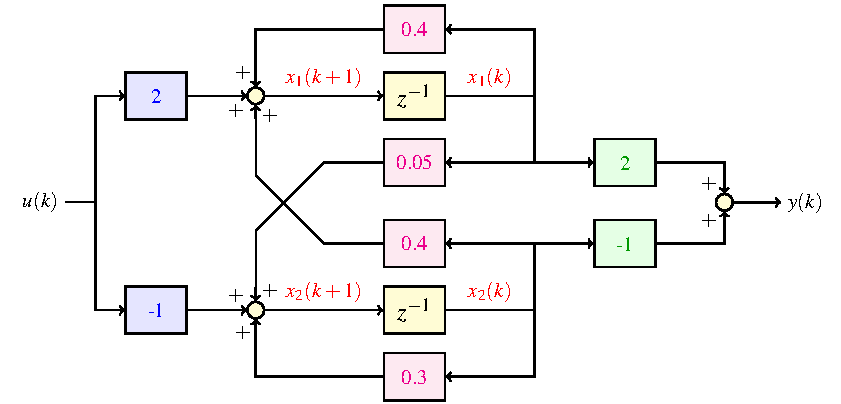
\includegraphics[width=0.85\columnwidth]{./Unit-03/img/PS01-ex02-fig07.pdf}
           \end{center}}
\end{frame}

\begin{frame}
\frametitleTC{Proposed exercise 02}
\framesubtitleTC{Try this at home, ask questions next time if needed}
\myPause
 Take the same system as in the previous proposed exercise, i.e.,
 \begin{displaymath}
  A = \begin{bmatrix} 0.5 & 0 \\ 2 & -0.3 \end{bmatrix}, \quad
  b = \begin{bmatrix} 1 \\ 0 \end{bmatrix}, \quad
  c = \begin{bmatrix} 0 & 4 \end{bmatrix}, \quad
  d = 1,
 \end{displaymath}
 and turn it into a block diagram.\\ \myPause
 \vspace{5mm}Remark: in this case you will see a \TC{direct feedthrough} from $u$ to $y$,\\
 because $d \neq 0$. 
\end{frame}

\begin{frame}
\frametitleTC{Takeaways}
\framesubtitleTC{from exercise 02 (and the proposed one)}
\myPause
 \begin{itemize}[<+-| alert@+>]
 \item Generalise the situation with compact matrix notation (thick lines are vectors):
       \begin{center}
        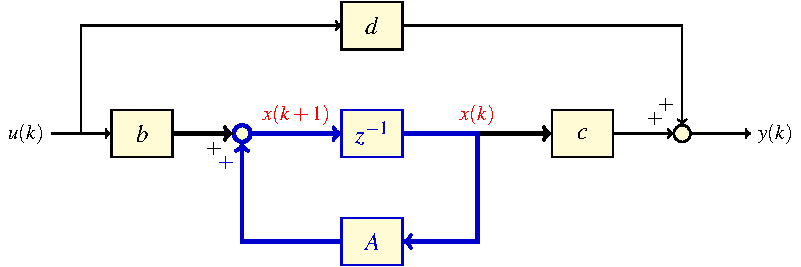
\includegraphics[width=0.65\columnwidth]{./Unit-03/img/PS01-ex02-takeaway-FBscheme.pdf}
       \end{center}
 \item Do you see the \textcolor{blue!80!black}{feedback loop} inherently inside the system?
 \item Feedback is not ``an invention for control''; it is an integral part\\
       of how nature works!
 \end{itemize}
\end{frame}

\begin{frame}
\frametitleTC{Takeaways}
\framesubtitleTC{from exercise 02 (and the proposed one)}
\myPause
 \begin{itemize}[<+-| alert@+>]
 \item Get acquainted with the $(k,k-1)$ and the $(k+1,k)$ ways of writing a DT system,\\
       and always pay attention to which symbol is what.
 \item In particular, the $u$ in the state equation is NOT at the same instant as that\\
       in the output equation, no matter how the system is written.
 \item \vspace{4mm}As feedback is a powerful weapon, ``slight'' approximations as taking\\
       the previous input of a block and not the current, or \emph{vice versa},\\
       can in fact be devastating...
 \item ...and without a system-theoretical analysis, this is impossible\\
       to figure out before the system is run --- i.e., possibly, broken.
 \end{itemize}
\end{frame}



